\documentclass[english]{article}
\usepackage[T1]{fontenc}
\usepackage[utf8]{inputenc}
\usepackage{babel}
\usepackage[unicode=true,pdfusetitle,
 bookmarks=true,bookmarksnumbered=false,bookmarksopen=false,
 breaklinks=true,pdfborder={0 0 1},backref=false,colorlinks=false]
 {hyperref}
\usepackage{tabularx}
\usepackage{graphicx}
\graphicspath{{images/}}
\usepackage{svg}
\usepackage{float}
\usepackage{titling}
\renewcommand{\arraystretch}{1.4}

\pretitle{%
	\begin{center}
		\LARGE
		
\includegraphics[width=250pt]{../other/Logo_blu.png}\\[\bigskipamount]~\\[\bigskipamount]
	}
\posttitle{\end{center}}

\begin{document}

\title{Politecnico di Milano\\
 A.A. 2016–2017 \\
Software Engineering 2: “PowerEnJoy” \\
\emph{Design Document}}

\author{Pietro Ferretti, Nicole Gervasoni, Danilo Labanca}
%\date{December 11, 2016}
\maketitle

\newpage

\tableofcontents{}

\newpage

\section{Introduction}

\subsection{Purpose}

\paragraph{}
"The purpose of this document is to provide a complete and detailed description and specification of a digital management system for PowerEnJoy, an electric car sharing service. This document will
illustrate functional and non-functional requirements of the software to-be, outlining costraints, showing potential user interfaces for the software, and explaining the domain assumptions made. Additionally, at the end of the document we will present an Alloy model to further specificate the world and environment our system will have to manage."

% scrivere a cosa serve il DD

% "descriviamo l'architettura del futuro sistema"
% "design del software"


\subsection{Scope}

% ricordiamo cos'è powerenjoy
% le principali cose che gli utenti possono fare

\paragraph{}
text here

\paragraph{}
more text here

\paragraph{}
....

\newpage
\subsection{Definitions, Acronyms, Abbreviations}

% vanno tolte le definizioni che non vengono usate in questo documento
% e aggiunte quelle in più

\subsubsection{Definitions}

\begin{itemize}
\item{\textit{Guest}: a person that is not registered to the system.}
\item{\textit{User}: a person that is registered to the system. Users can log in to the system with their email or username and their password. Their first name, last name, date of birth, driving license ID are stored in the database.}
\item{\textit{Safe area}: a location where the user can park and leave the car. Users can end their ride and park temporarily only in these locations. The set of safe areas is predefined by the system.}
\item{\textit{Power grid station}: a place where cars can be parked and plugged in. While a car is plugged in a power grid station its battery will be recharged. Power grid stations are by definition safe areas.}
\item{\textit{Available car}: a car that is currently not being used by any user, and has not been reserved either. Available cars are in good conditions (not dirty nor damaged) and don’t have dead batteries.}
\item{\textit{Reservation}:
	\begin{itemize}
		\item{the operation of making a car reserved for a user, i.e. giving permission to unlock and use the car only for that user, forbidding reservations by other users.}
		\item{the time period between the moment a reservation is requested and the moment the user unlocks the car, or the reservation is canceled.}
	\end{itemize}
}
\item{\textit{Ride}: the time period from the moment a reserved car is unlocked to the moment the user notifies that he wants to stop using the car and closes all the doors. A ride doesn’t stop when a car is temporarily parked, but continues until the user chooses to leave the car definitely.}
\item{\textit{Possession}: users that have reserved and unlocked a car are said to have possession of the car. While a user has possession of a car they are the only person that can drive it, lock or unlock it, and no other person can take possession of it until the user frees it. Users lose possession of a car when their ride ends.}
\item{\textit{Temporary parking}: the act of parking a car in a safe area and, after notifying the system, locking it and leaving it for a finite amount of time. The user that does this retains the right to use the car and can unlock it later to use it again.}
\item{\textit{Bill}: a record of the money owed by the user at the end of a ride.}
\item{\textit{Outstanding bill}: a bill that hasn’t been paid yet. }
\item{\textit{Suspended user}: a user that cannot reserve or use cars. Usually users are suspended because they have outstanding bills.}
\item{\textit{Payment method}: a way to transfer money from the user to the system. Our system will only accept credit cards and online accounts like Paypal.}
\item{\textit{Payment API}: an interface to carry out money transactions, offered by the external provider associated to the payment method used (e.g. a bank).}
\item{\textit{CAN bus}: a vehicle bus standard designed to allow micro controllers and devices to communicate with each other.}
\end{itemize}

\subsubsection{Acronyms}
\begin{itemize}
\item{\textbf{DD}: Design Document}
\item{\textbf{RASD}: Requirements Analysis and Specification Document}
\item{\textbf{DB}: Database}
\item{\textbf{CVV}: Card Verification Value}
\item{\textbf{DOB}: Date of birth}
\item{\textbf{PGS}: Power Grid Station}
\item{\textbf{GPS}: Global Positioning System}
\item{\textbf{CAN bus}: Controller Area Network bus}
\end{itemize}

\subsubsection{Abbreviations}
\begin{itemize}
\item{\textbf{[Gx]}: Goal}
\item{\textbf{[RE.x]}: Functional Requirement}
\item{\textbf{[UC.x]}: Use Case}
\end{itemize}

\subsection{Reference Documents}

\begin{itemize}
	\item{IEEE Std. 1016-2009, “IEEE Standard for Information Technology -- Systems Design -- Software Design Descriptions”}
	\item{ISO/IEC/IEEE Std. 42010:2011, “Systems and software engineering -- Architecture Description”}
	\item{Specification document: “Assignments AA 2016-2017.pdf”}
\end{itemize}

\newpage{}

\subsection{Document Structure}

%% DA RILEGGERE

This document is structured as follows:
\begin{itemize}
\item{\textbf{Section 1 -- Introduction:} this section introduces the design document. It contains
	a justification of his utility and indications on which parts are covered in
	this document that are not covered by the RASD.}
\item{\textbf{Section 2 -- Architectural Design:} this section is divided into more parts:
	\begin{itemize}
		\item{\textbf{Overview:} this section shows a high-level view of our system's architecture.}
		\item{\textbf{Component View:} this section gives a more detailed (in-depth) view of the components of the application and how they communicate.}
		\item{\textbf{Deployment View:} this section shows the way the components will be deployed to run our application.}
		\item{\textbf{Runtime View:} in this section we use sequence diagram to show the flow of the most important functionalities of the system.}
		\item{\textbf{Component Interfaces:} the interfaces between the components are presented in this section.}
		\item{\textbf{Selected Architectural Styles and Patterns:} this section explains the architectural choices taken during the creation of the application.}
		\item{\textbf{Other Design Decisions}}
	\end{itemize}}
\item{\textbf{Section 3 -- Algorithm Design:} this section describes the most critical parts via some algorithms. Pseudo code is used in order to hide unnecessary implementation details in order to focus on the most important parts.}
\item{\textbf{Section 4 -- User Interface Design:} this section presents mockups and user experience explained via UX and BCE diagrams.}
\item{\textbf{Section 5 -- Requirements Traceability:} this section aims to explain how the requirements identified in the RASD are linked to design elements.}
\item{\textbf{Effort Spent} }
\item{\textbf{References} }
\item{\textbf{Revisions} }
\end{itemize}

\newpage

\section{Architectural Design}

\subsection{Overview}

\subsection{Component View}

% inserire immagine component view

% spiegazione veloce immagine

\newpage
\subsection{Deployment View}

% inserire immagine deployment view
\begin{figure}[H]
	\centering
	\makebox[\textwidth][c]{
		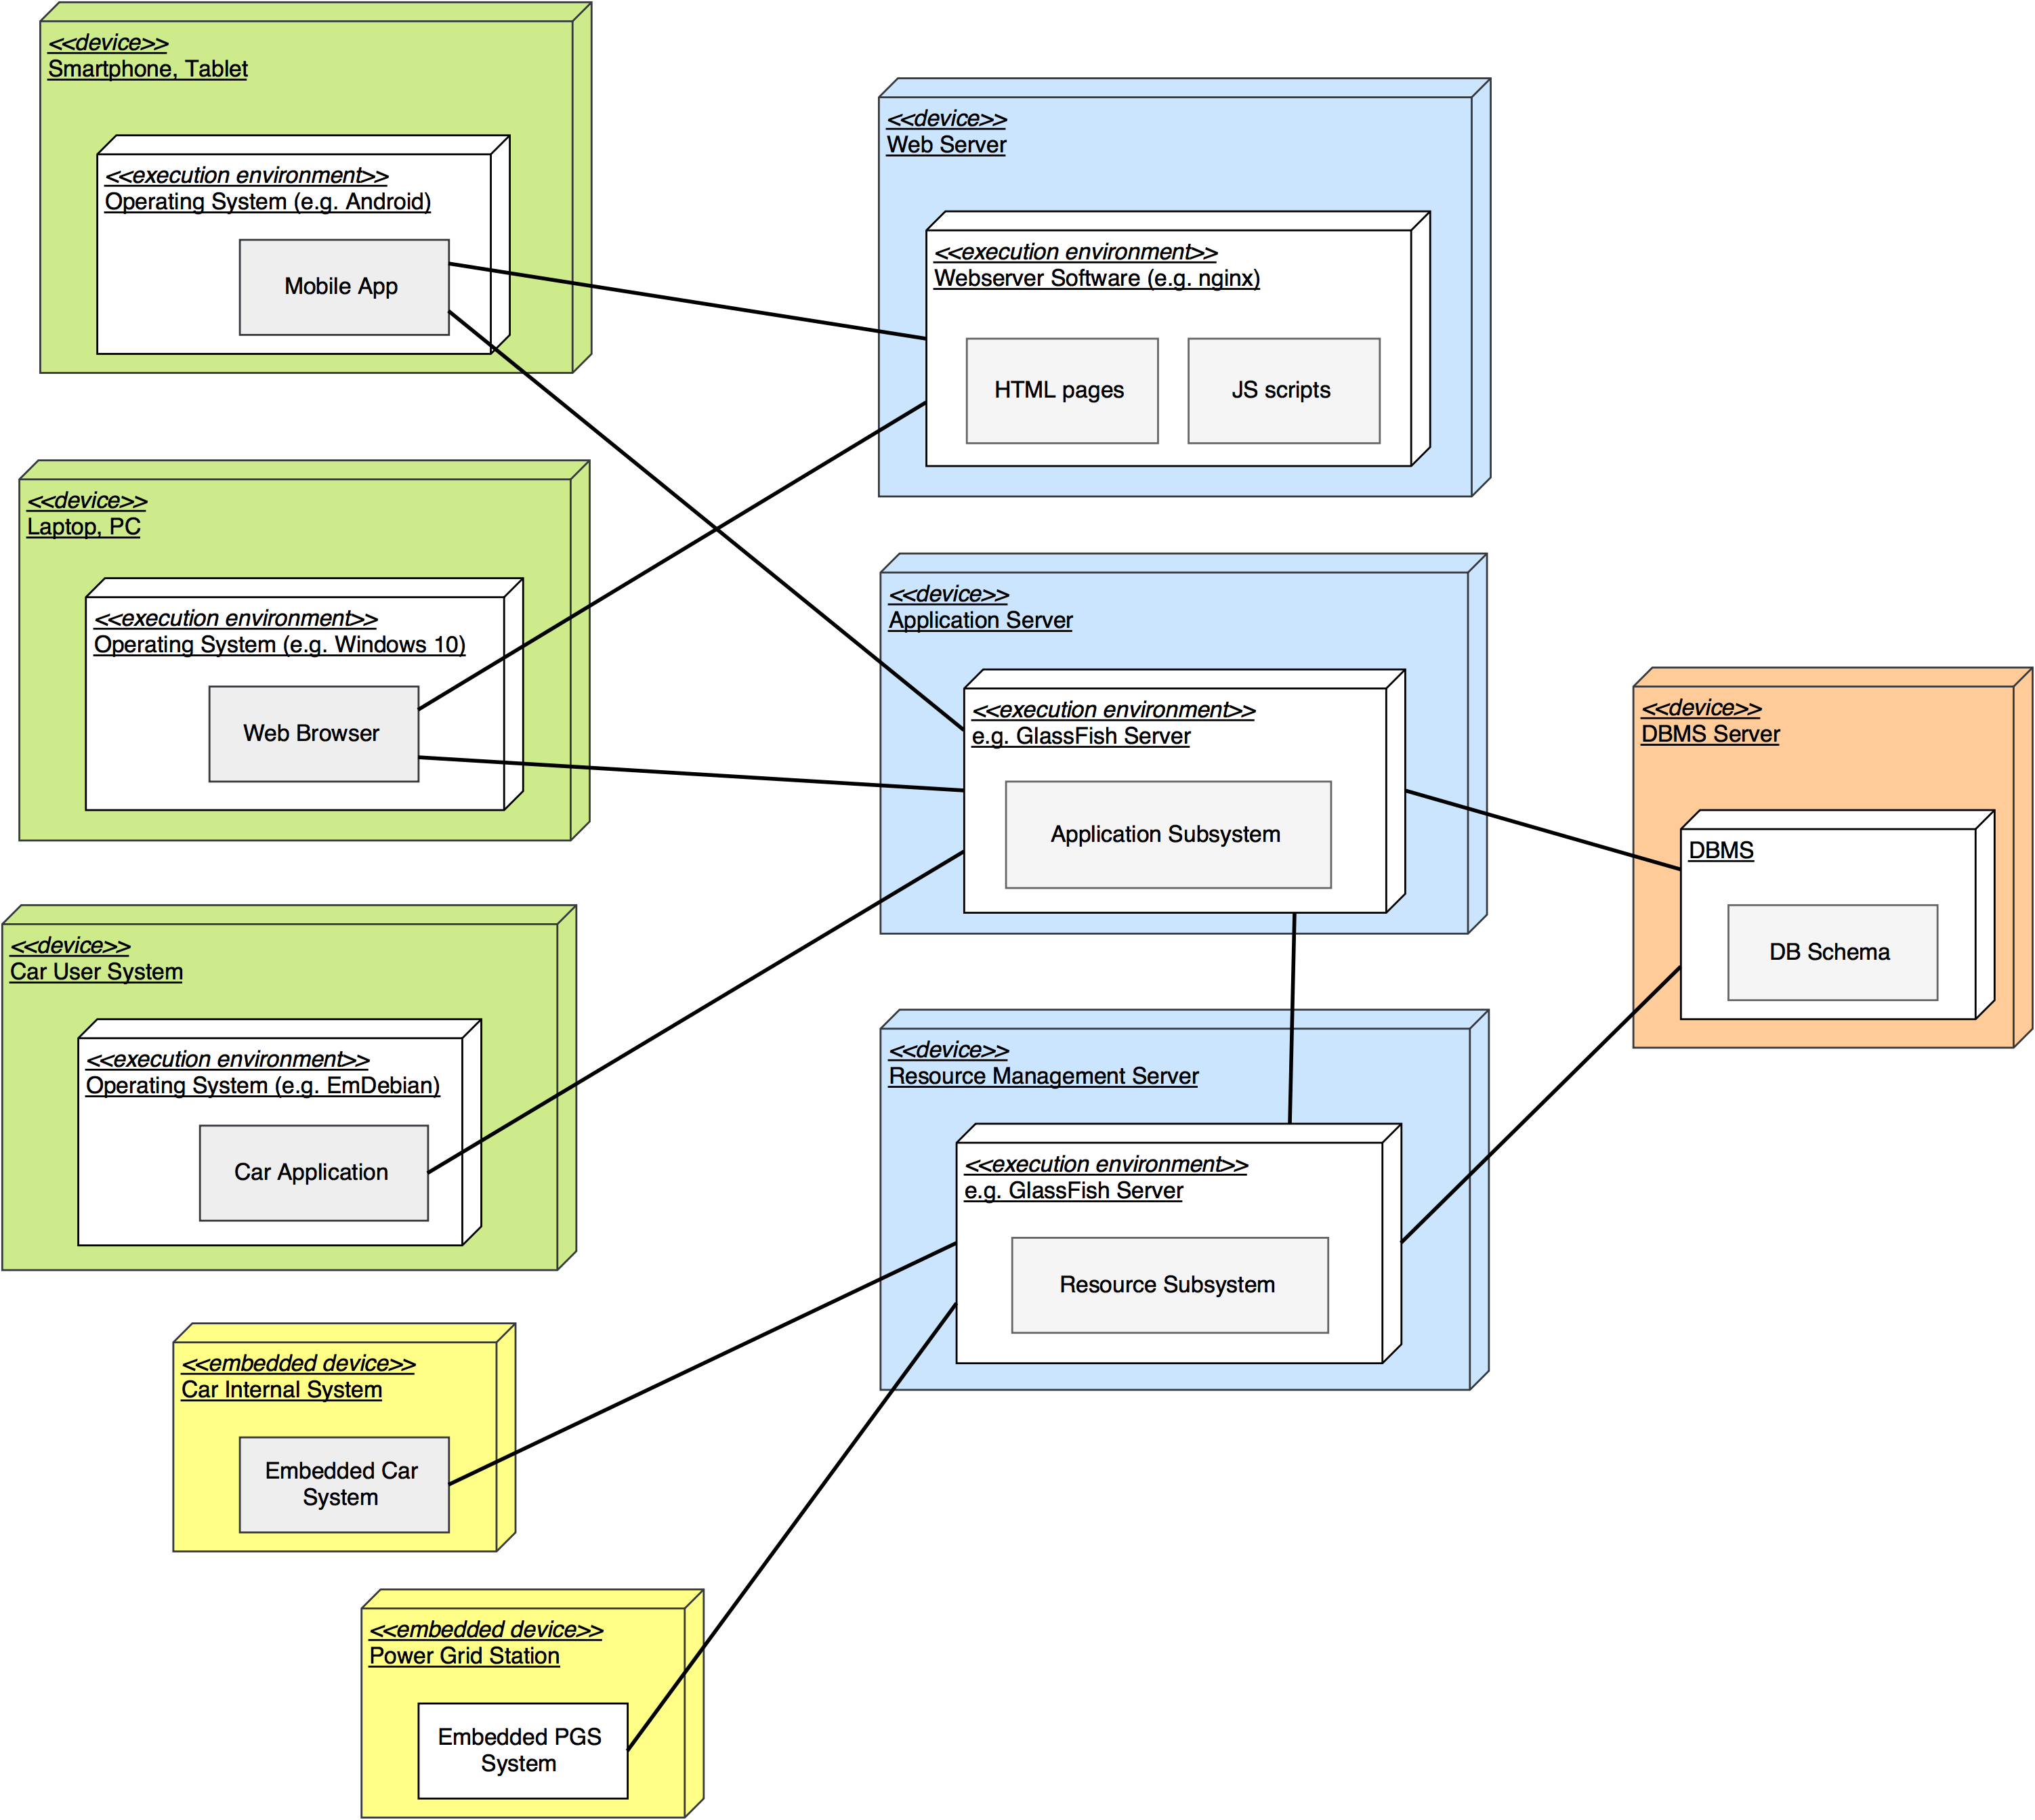
\includegraphics[width=450pt]{deployment_diagram.png}
	}
	\caption{Deployment Diagram}
	\label{deploymentdiagram}
\end{figure}

% spiegazione veloce immagine
tre tier: client, business logic, database

client:
- app e browser si collegano al web server per avere le pagine web, poi si collegano all'application server per raccogliere i dati
- l'applicativo sulla macchina non è basato sul web e si collega direttamente all'application server per avere tutto
- esiste un "resource management server" che raccoglie informazioni (gps, ecc.) dalle macchine e disponibilità posti dalle PGS
- l'application server inoltre può inviare comandi alle macchine tramite il resource server
- application server e resource server sono collegati al DBMS che contiene tutto in tempo reale
% --> caching delle informazioni su server, poi una transazione ogni tanto?

\subsection{Runtime View}

% sequence diagrams

\subsection{Component Interfaces}

\subsection{Selected Architectural Styles and Patterns}

% Architecture Overall?

\subsubsection{Protocols}
% rest?

\subsubsection{Patterns}
% mvc
% facade
% client-server
% event-driven architecture
% adapter?

\subsection{Other Design Decisions}

\newpage

\section{Algorithm Design}

% "Java-like pseudo-code"

\newpage

\section{User Interface Design}

\subsection{Mockups}
% rimandare al RASD

\subsection{UX Diagrams}

\subsection{BCE Diagrams}

\newpage

\section{Requirements Traceability}

\newpage

\section{Effort Spent}

\newpage

\section{Revisions}

\subsection{Changelog}
\begin{itemize}
  \item{}
\end{itemize}
\end{document}
